\documentclass[11pt, notitlepage,  letterpaper]{article}


%% Horizontal Lengths - Max 6.5
\setlength{\footskip}{0.5in}
\setlength{\hoffset}{0in}
\setlength{\oddsidemargin}{-.2in}
\setlength{\evensidemargin}{-.2in}
%\setlength{\textwidth}{6.9in}
\setlength{\textwidth}{6.6in}

%% Vertical Lengths - Max 9.0
\setlength{\headheight}{0in} \setlength{\topskip}{0in}
\setlength{\voffset}{0in} \setlength{\topmargin}{0.5in}
\setlength{\textheight}{8.5in}

%\usepackage{fancyheadings}

\usepackage{url}
\usepackage[]{epsfig,amsmath}[]
%\usepackage{doublespace}

%\pagestyle{headings}
%\pagestyle{fancy}
\pagenumbering{arabic}

\renewcommand{\baselinestretch}{1.15}

%%%%%%%%%%%%%%%%%%%%%%%%%%%%%%%%%%%%%%%%%%%%%%%%%%%%%%%%%%%%%%%%%%%%%%
% New definitions and commands
\newtheorem{define}{Definition}[section]
\newtheorem{theorem}[define]{Theorem}
\newtheorem{question}[define]{Question}
\newtheorem{problem}[define]{Problem}


%**************************************

\begin{document}
%\title{{\normalsize Fall 2003, Semester research;}\\
\title{
{Solving the Poisson Partial Differential Equation}\\
{using Spectral Polynomial Methods }
}

 \vfill
\author{Seungkeol\ Choe \thanks{Computational Engineering and Science Program, University of Utah}}

\renewcommand{\today}{April 18th, 2004}

\maketitle

\begin{abstract}
In this report, we present a spectral polynomial method for
solving the Poisson equation with Dirichlet and Neumann boundary
conditions respectively on a one dimensional compact interval. We
can control the number, size of elements, and order of
approximating polynomials to obtain accurate solutions with faster
convergence than the classical finite element method. We present a
spectral Fourier method for solving a Poisson equation with the
same boundary conditions on an two dimensional annulus domain. By
using the tensor product between one dimensional spectral bases
and Fourier bases, we apply the high-order method to radius
direction and the fast Fourier transform to angular direction.
\end{abstract}

%\noinden {\bf Keywords: Spectral Element Methods, Poisson Equation}
\clearpage

\tableofcontents

%-------------------------------------------------------------------------------
\clearpage

%\begin{spacing}{2}

\section{Introduction}

%\{ {\it  sp1d\_ch1.tex} \}

The spectral method is a numerical scheme for approximating the
solution of partial differential equations. It has developed
rapidly in the past three decades and has been applied to
numerical simulation problems in many fields.

One reason for its broad and fast acceptance is its use of various
systems of infinitely differentiable basis functions as trial
functions. By choosing an appropriate orthogonal system based on
domain of orthogonality, we can apply the method to periodic and
non-periodic problems, as well as problems defined on various
domains, such as compact domain, half/all intervals.

Another advantage of the spectral method is its high accuracy. In
particular, the spectral polynomial method allows control of both
the resolution of element size and the order of approximation.
This results in exponential convergence, which is a marked
improvement over classical finite difference and other purely
element methods.

For solving the problem, we discretize the domain and obtain the
following approximation of infinite series. A function $u$ is
represented via a truncated series expansion as follows:
\begin{equation}
\label{solapprx}
u \approx u_N = \sum_{n=0}^{N} \hat u_n \phi_n,
\end{equation}
where $\phi_n$ are the basis functions. In general the Chebyshev
polynomials $T_n$ or the Legendre polynomials $L_n$ or another
member of the class of Jacobi polynomials $P_n^{\alpha, \beta}$
are employed as basis functions.

In choosing proper basis function, we apply the following 3
characteristics to the candidate basis.
\begin{itemize}
\item {\bf Numerical Efficiency} After discretization,
the choice of basis affects complexity of mass matrix. Moreover we
need consider the efficiency in solving the system of linear
equations. For example, using the monomials $\{x^k\}_{k=0}^{N}$
result in the matrix whose non-zero component are the half. But
its inverse matrix is full and the cost of inverting is dominant.
In contrast, the Legendre polynomial basis composes diagonal mass
matrix and its inverse matrix can be calculated very efficiently.
\item {\bf Conditioning} If a matrix system is ill-conditioned
the round-off error in the matrix system can lead to large errors
in the solution. Furthermore the number iteration required in
inverting the matrix using iterative solver can be increase by the
condition number. The condition number of monomials and Lagrange
polynomial are close to $10^p$, for the polynomial order $p$. But
Legendre polynomial has condition number $2P+1$. This condition
also affects the degree of linear independence of each basis
function.
\end{itemize}

This project seeks to study the fundamental theory of spectral
method, problems, solvability, and to obtain its constructive
procedure to apply the method to various application problems. By
checking solutions obtained via the spectral method against exact
solutions, we can validate the method and see how much we can save
the effort on discretisation of domain to achieve the same degree
of accuracy in comparison to classical element methods.

In chapter 2, I investigate spectral method solutions for the
forward Poisson problem with Dirichlet and Neumann boundary
condition on each end of one dimensional interval domain. In
chapter 3, I investigate the spectral polynomial method and
Fourier method for solving the forward Poisson problem with
Dirichlet and Neumann boundary condition on inner and outer
boundary circles respectively. Our approach utilizes spectral
polynomial element and Fourier method in tensor product form. As
an conclusion we present the result of numerical solution and its
convergence by h/p adaptive control.

\subsection{Poisson Equation}

Science and engineering disciplines are generally interested in
systems of continuous quantities and relations. This project
focuses on solutions of the Poisson equation, which appears in
various field such as electrostatics, magnetics, heat flow,
elastic membranes, torsion, and fluid flow.

For example, electrostatics, the governing equation appears as
Gauss's law in differential form \cite{Johnson}:
\begin{equation}
\nabla \cdot \mathbf{E} = 4 \pi \rho
\end{equation}
which indicates that the charge within a closed spherical surface
is related to the electric field \textbf{E} normal to surface
element where $\rho$ is a charge density.

Since it is known in electrostatics that the electric field \textbf{E} is conservative, \textbf{E} is a form of gradient of a scalar potential $\Phi$,
\begin{equation}
\mathbf{E} = - \nabla\Phi.
\end{equation}
With these two relationships, we obtain a Poisson equation
\begin{equation}
\nabla^2\Phi = -4\pi\rho.
\end{equation}


In this report, the one-dimensional Poisson equation is defined as

\begin{equation}
\label{poisson1} L(u) \equiv  \frac{d^2}{dx^2} u + f = 0.
\end{equation}
where $u$ and $f$ are defined on $\Omega$.

In pointwise viewpoint, the one dimensional Poisson equation
(\ref{poisson1}) is written as
\begin{equation}
\label{poisson2} L(u)(x) \equiv \frac{d^2}{dx^2} u(x) + f(x) = 0,
\end{equation}
for all $x$ in $(a, b)$.

\subsection{Method of Weighted Residuals}
According to the Weierstrass approximation theorem, for any given
real valued continuous solution $u$ on a compact interval $[a, b]$
we can obtain real polynomial function $p$ of certain degree such
that $p$ uniformly approximates $u$. Although the result of
convergence at each point is within a predefined error bound, this
does not satisfy the requirement that we need to acquire an
accurate solution on a specific situation. By imposing certain
restrictions, we can obtain a formulation that satisfies the
requirement.

To describe this, we set a general linear differential equation on $\Omega$.
\begin{equation}
\label{pde1} L(u) = 0.
\end{equation}
with appropriate initial and boundary conditions. Under certain
restriction,  we assume that the true solution $u(x)$ can be
approximated by a finite series expansion of the form:
\begin{equation}
\label{sol1} u^{\delta}(x) = \sum_{i=0}^{N_{dof}-1} \hat u_i
\Phi_i(x),
\end{equation}
where $\Phi_i(x)$ are polynomial trial functions and $\hat u_i$
are $N_{dof}$ unknown coefficients. We assume the following:
\begin{eqnarray}
    \hat u_0  &=& \mathcal{G}_{D} \qquad \mbox{: Dirichlet Boundary Value}, \\
    \Phi_0(a) &=& 1,  \Phi_{N_{dof}-1}(b) = 1 \qquad \mbox{where $a, b$ are the boundary of domain $\Omega$}\\
\end{eqnarray}
We then define a non-zero residual $R$ by:
\begin{equation}
R(u^{\delta}) = L(u^{\delta}).
\end{equation}

Define a set of functions, $H^1(\Omega)$  and a norm
$||\cdot||_{H^1(\Omega)}$ on the space as follows:
\begin{eqnarray}
H^1(\Omega) &=& \{v \in L^2(\Omega) : \frac{d}{dx}v \in L^2(\Omega)\}, \\
||v ||_{H^1(\Omega)} &=& \left[ \int_{\Omega}v(x)^2 + \frac{d}{dx}v(x)^2 dx \right]^{\frac{1}{2}}, \quad v \in H^1(\Omega).
\end{eqnarray}

We define an inner-product $\langle \cdot, \cdot \rangle$ over
$H^1(\Omega)$  as follows:
\begin{equation}
\label{functional}
\langle u, v \rangle = \int_{\Omega} u(x) \cdot v(x) dx,
\end{equation}

This method is restricted to test functions, $v(x)$ that satisfy:
\begin{equation}
\langle v, R \rangle = 0.
\end{equation}

For example, in the collocation method, the $j^{th}$ test function
is the Dirac delta function which evaluates to a collocation point
$x = x_j$. Then we have
\begin{equation}
0 = \langle \delta_j, R \rangle = \int_{\Omega} R(u^{\delta})(x)\delta_j(x)dx = R(u^{\delta})(x_j) = L(u^{\delta})(x_j).
\end{equation}

Other possible test functions are examined in \cite{Karniadarkis}.


\clearpage
\section{Spectral Polynomial Elements Method on an Interval}

\subsection{Mathematical Formulations}
%\{ {\it  sp1d\_ch2.tex} \}

To formulate Spectral Element Methods, we presume the following boundary conditions to the equation (\ref{poisson1}) and (\ref{poisson2}).
\begin{eqnarray}\label{bdycond}
    u(a) &=& {\mathcal G}_D \qquad \mbox{ : Dirichlet Condition}\\
    \frac{d}{dx}u(b) &=& \mathcal{G}_N \qquad \mbox{ : Neumann Condition}.
\end{eqnarray}

Multiplying equation (\ref{poisson1}) and by integration by part,
\begin{eqnarray}
\int_a^b v(x)\frac{d^2}{dx^2}u(x) dx &+& \int_a^b v(x) f(x) dx = 0,\\
\label{weakform1}
\int_a^b \frac{d}{dx}v(x)\frac{d}{dx}u(x)dx &=& \int_a^b v(x) f(x) dx + \left[v \frac{d}{dx}u\right]_a^b,
\end{eqnarray}
for $u, v$ being sufficiently smooth.

Define a set $H^1(\Omega)$ of functions and a norm $||\cdot||_{H^1(\Omega)}$ on it as follows:
\begin{eqnarray}
H^1(\Omega) &=& \{v \in L^2(\Omega) : \frac{d}{dx}v \in L^2(\Omega)\}, \\
||v ||_{H^1(\Omega)} &=& \left[ \int_{\Omega}v(x)^2 + \frac{d}{dx}v(x)^2 dx \right]^{\frac{1}{2}}, \quad v \in H^1(\Omega).
\end{eqnarray}

Consider solutions to problem (\ref{poisson1}) where the forcing function $f$ is well defined in the sense that
$\int_a^b v f + \left[ v u^{\prime} \right]_a^b < \infty$. Therefore we only consider trial solutions to equation (\ref{weakform1}) which lie in $H^1(\Omega)$ and satisfy the Dirichlet boundary condition. We can define the trial space by

\begin{equation}
\mathcal{X} = \{u\in H^1|u(a) = {\mathcal G}_D\}.
\end{equation}
Similarly, the space of all test functions are defined by being homogeneous on all Dirichlet boundaries, that is
\begin{equation}
\mathcal{V} = \{v\in H^1|v(a) = 0\}.
\end{equation}

For numerical approximation, we select finite subspace $\mathcal{X}^{\delta} (\subset \mathcal{X})$ and $\mathcal{V}^{\delta} (\subset \mathcal{V})$ for which equation (\ref{weakform1}) holds. In particular, we can define $\delta$ by the choice of two different discretization approaches : Element size or Polynomial order. The formulation for the weak solution (\ref{weakform1}) can be stated as:

Find $u^{\delta} \in \mathcal{X}^{\delta}$, such that
\begin{equation}
\int_a^b \frac{d}{dx}v^{\delta}(x)\frac{d}{dx}u^{\delta}(x)dx = \int_a^b v^{\delta}(x) f(x) dx + \left[v^{\delta} \frac{d}{dx}u^{\delta}\right]_a^b, \qquad v^{\delta} \in \mathcal{V}^{\delta}.
\end{equation}




%we find $u^{\delta}$ such that

%\begin{equation}
%\label{weakabs}
%\langle L(u), v \rangle = \langle \nabla^2 u, v \rangle + \langle f, v \rangle =\int_a^b \frac{d^2}{dx^2} u(x) v(x) dx + \int_a^b f(x) v(x) dx = 0,
%\end{equation}
%where by the definition of Galerkin method, $v$ is function generated by linear combination from a set of basis functions on which $u$ defined in $\left[a, b\right]$.

%--------------------------------------------------------------------------
\subsection{Basis Functions}

The spectral approximation of solution $u$ is generally represented as
\begin{equation}\label{genrep}
u(x) = \sum_{i=0}^{N_{dof-1}} \hat u_i\Phi_i(x)
\end{equation}
on $[a, b]$. To construct the global basis functions $\{\Phi_i(x)\}_{i=0}^{N_{dof-1}}$, each $\Phi_i$ is represented by the linear combination of local basis functions $\phi_i$ on each element in $[a, b]$, say $\Omega^e$.

We define the local basis functions ${\phi_i}$ on $[-1, 1]$ to be a real valued function with Jacobi polynomial of $\alpha = 1$ and $\beta = 1$ $\{P_i^{1,1}\}$ as follows:
\begin{equation}
\label{locbasis}
  \phi_i(\xi) =\left \{
    \begin{array}{ll}
    \frac{1-\xi}{2}, & i=0 \\
    \left(\frac{1-\xi}{2}\right)\left(\frac{1+\xi}{2}\right)P_{i-1}^{1,1}(\xi),
    \qquad &1 \le i \le P-1 \\
    \frac{1+\xi}{2}, & i=P \\
    \end{array}   \right.
\end{equation}
for all $\xi$ in $[-1, 1]$.

Then on a single standard element $[-1, 1]$, the approximation $u(\xi)$ is represented as
\begin{equation}\label{locrep}
u(\xi) = \sum_{i=0}^{P_e} \hat u_{i}^{e}\phi_i(\xi),
\end{equation}
for $\xi$ in $[-1, 1]$.

The local basis function $\phi_i^e$ on general element $[x_1, x_2]$ is defined by the change of variable for $\phi_i$ between two interval $[x_1, x_2]$ and $[-1, 1]$.

%--------------------------------------------------------------------------
\subsection{Spectral Polynomial Method in an Element}

We apply the basis representation (\ref{locrep}) to weak formulation (\ref{weakform1}) with the same test function $\{\phi_q\}$, then we obtain the following:
\begin{equation}\label{locmat}
 - \sum_{p=0}^{P_e} \hat u_p^e \langle \frac{d^2}{dx^2} \phi_p, \phi_q \rangle = - \langle \frac{d^2}{dx^2} \sum_{p=0}^{P_e} u_p^e \phi_p, \phi_q \rangle = \langle f, \phi_q \rangle
\end{equation}
for $q = 0, \cdots, P_e$ where $P_e$ is the order of polynomial on local element $\Omega^{e}$, say $\left[ x_1, x_2 \right]$.

By integration by part, we can use the fact that
\begin{equation}\label{intpart}
\langle \frac{d^2}{dx^2} \phi_p, \phi_q \rangle = \left[ \frac{d}{dx}\phi_p(x) \phi_q(x) \right]_{x_1}^{x_2} - \langle \frac{d}{dx} \phi_p, \frac{d}{dx} \phi_q \rangle.
\end{equation}

by applying (\ref{intpart}) to (\ref{locmat}), we obtain
\begin{eqnarray}\label{locmat}
&- \left[\frac{d}{dx}u(x)\phi_q(x) \right]_{x_1}^{x_2} + \sum_{p=0}^{P_e} \hat u_p^e \langle \frac{d}{dx} \phi_p, \frac{d}{dx} \phi_q \rangle
%= - \left[ \sum_{p=0}^{P_e} \hat u_p^e \frac{d}{dx}\phi_p(x) \phi_q(x) \right]_{x_1}^{x_2} + \sum_{p=0}^{P_e} \hat u_p^e \langle \frac{d}{dx} \phi_p, \frac{d}{dx} \phi_q \rangle \\
= - \sum_{p=0}^{P_e} \hat u_p^e \langle \frac{d^2}{dx^2} \phi_p, \phi_q \rangle  = \langle f, \phi_q \rangle \\
&\sum_{p=0}^{P_e} \hat u_p^e \langle \frac{d}{dx} \phi_p, \frac{d}{dx} \phi_q \rangle = \langle f, \phi_q \rangle + \left[\frac{d}{dx}u(x)\phi_q(x) \right]_{x_1}^{x_2}
\end{eqnarray}
for $q = 0, \cdots, P_e$.

In matrix form we obtain the following the system of equations for local coefficients and modes:
Note that $\phi_q(x_1) = \delta_{q,1}$, $\phi_q(x_2) = \delta_{q, P_e}$ and the orthogonality on $\{\phi_q\}_{q=1}^{P_e-1}$ .
\begin{eqnarray}
\label{localsystem}
\begin{bmatrix}
    \phi_{0,0}^e   & 0            & \cdots & 0                    & \phi_{0,P_e}^e      \\
    0              & \phi_{1,1}^e & \cdots & 0                    & 0                   \\
    \vdots         & \vdots       & \ddots & \vdots               & \vdots              \\
    0              & 0            & \cdots & \phi_{P_e-1,P_e-1}^e & 0                   \\
    \phi_{P_e,0}^e & 0            & \cdots & 0                    & \phi_{P_e,P_e}^e    \\
\end{bmatrix}
\begin{bmatrix}
    {\hat u^e}_{0}      \\
    {\hat u^e}_{1}      \\
    \vdots              \\
    {\hat u^e}_{P_e-1}  \\
    {\hat u^e}_{P_e}    \\
\end{bmatrix}
=
\begin{bmatrix}
    f^e_{0}     \\
    f^e_{1}     \\
    \vdots      \\
    f^e_{P_e-1} \\
    f^e_{P_e}   \\
\end{bmatrix}
+
\begin{bmatrix}
    0       \\
    0       \\
    \vdots  \\
    0       \\
    1       \\
%    \phi_{0}(x_2)     \\
%    \phi_{1}(x_2)     \\
%    \vdots            \\
%    \phi_{P_e-1}(x_2) \\
%    \phi_{P_e}(x_2) \\
\end{bmatrix}
u^{\prime}(x_2)
-
\begin{bmatrix}
    1       \\
    0       \\
    \vdots  \\
    0       \\
    0       \\
%    \phi_{0}(x_1)     \\
%    \phi_{1}(x_1)     \\
%    \vdots            \\
%    \phi_{P_e-1}(x_1) \\
%    \phi_{P_e}(x_1) \\
\end{bmatrix}
u^{\prime}(x_1)
\end{eqnarray}
where $\phi_{p,q} = \langle \frac{d}{dx} \phi_p, \frac{d}{dx} \phi_q \rangle$, $f_q^e = \langle f, \phi_q \rangle$, $p, q = 0, \ldots, P_e $.


\subsection{Global Assembly/Direct Stiffness Summation} As seen on
equation (\ref{sol1}), we have the finite element approximation
$u^{\delta}$ in terms of the global modes. Moreover, we can
represent $u^{\delta}$ in terms of linear combination of local
modes ${\phi_p^e}$ :
\begin{equation}
\label{sol2} u^{\delta}(x) = \sum_{i=0}^{N_{dof-1}}\hat u_i \Phi_i(x) = \sum_{e=1}^{N_{el}}\sum_{p=0}^{P_e}{\hat u}_p^e \phi_p^e(\xi),
\end{equation}
where in this case $P_e$ is the polynomial order of the expansion and $\phi_p^e(\xi)$ is reparametrization of local basis function general elements.

We have the following relationship between global and local coefficients $(\hat u_i,\hat u_i^e)$:
\begin{eqnarray}
\label{coefoverlap}
\hat u_0^1 &=& \hat u_0 \\
\hat u_{P_{e}}^{e} &=& \hat u_{0}^{e+1} = \hat u_r, \qquad e = 1, \ldots, N_{el}-1, \mbox{ for some } r \le N_{dof}-2, \mbox{ and}\\
\hat u_{P_{e}}^{e} &=& \hat u_r, \qquad \qquad e = N_{el},\quad r = N_{dof}-1.
\end{eqnarray}

When we determine $\hat u_i, i = 0, \ldots, N_{dof}-1$, this
property plays a role that we can reduce the size of system.

According to the orthogonality defined in $\{\phi_p^e\}$, the following relationships hold
\begin{equation}
\label{q0}\phi_{q,q}^e \hat u_q^e = f_q^e, \qquad q = 1, \ldots, P_e-1
\end{equation}
for every element $e$.

By the orthogonality in $\{\phi_p^e\}$ and the identity (\ref{coefoverlap}) we obtain the relationship below:

For adjacent elements $e_0=[x_0, x_1]$, $e_1=[x_1, x_2]$, and $e_1=[x_2, x_3]$ of polynomial order $P_0, P_1$, and $P_2$, respectively,
\begin{eqnarray}
\label{q1}  \phi_{P_0, 0}^0\hat u_0^0 + \phi_{P_0, P_0}^0 \hat u_{P_0}^0 &=& f_{P_0}^0 - u^{\prime}(x_1) \\
\label{q2}  \phi_{0, 0}^1\hat u_0^1 + \phi_{0, P_1}^1 \hat u_{P_1}^1     &=& f_{0}^1 + u^{\prime}(x_1) \\
\label{q3}  \phi_{P_1, 0}^1\hat u_0^1 + \phi_{P_1, P_1}^1 \hat u_{P_1}^1 &=& f_{P_1}^1 - u^{\prime}(x_2) \\
\label{q4}  \phi_{0, 0}^2\hat u_0^2 + \phi_{0, P_2}^0 \hat u_{P_2}^2     &=& f_{0}^2 + u^{\prime}(x_2)
\end{eqnarray}
(\ref{q1})$+$(\ref{q2}), (\ref{q3})$+$(\ref{q4}) give
\begin{eqnarray}
\label{q5}  -.5 \cdot \hat u_0^0 + 1 \cdot \hat u_{P_0}^0(=u_0^1) -.5 \cdot \hat u_{P_1}^1 &=& f_{P_0}^0 + f_{0}^1 \\
\label{q6}  -.5 \cdot \hat u_0^1 + 1 \cdot \hat u_{P_1}^1(=u_0^2) -.5 \cdot \hat u_{P_2}^2 &=& f_{P_1}^1 + f_{0}^2
\end{eqnarray}

By equation (\ref{q0}),(\ref{q5}), and (\ref{q6}) we can deduce
the system of global stiffness matrix showing the assembly of two
adjacent local element matrix system as follows:
\begin{eqnarray}
\label{localsystem}
&{\mathbf A \mathbf{\hat u} = \mathbf f} \mbox{ is defined by }
\end{eqnarray}
\begin{eqnarray*}
\begin{bmatrix}
    \ddots &\vdots  &\vdots &\vdots &\vdots &\vdots &\vdots &\vdots & \\
    \cdots0 &\phi_{P_0-1,P_0-1}^0   & 0     & 0     &\cdots & 0     & 0     & 0     &0\cdots    \\
    \cdots-.5\cdots0 & 0    & 1     & 0     &\cdots & 0     & -.5   & 0     &0\cdots \\
    \cdots0 & 0      & 0    &\phi_{1,1}^1   &\cdots & 0     & 0     & 0     &0\cdots \\
    \vdots &\vdots  &\vdots &\vdots &\ddots &\vdots &\vdots &\vdots &\vdots  \\
    \cdots0 & 0      & 0    & 0    &\cdots  &\phi_{P_1-1,P_1-1}^1   & 0     & 0   &0\cdots \\
    \cdots0 & 0      & -.5  & 0    &\cdots  & 0     &1      & 0     & 0\cdots-5\cdots \\
    \cdots0 & 0      & 0    & 0    &\cdots  & 0     &0      &\phi_{P_0,P_0}^2   & 0\cdots \\
           &\vdots  &\vdots &\vdots &\vdots &\vdots &\vdots &\vdots &\ddots
\end{bmatrix}
\begin{bmatrix}
    \vdots      \\
    {\hat u_{P_0-1}^0}  \\
    {\hat u_0^1}\\% = {\hat u_{P_0}^0} \\
    {\hat u_1^1}\\
    \vdots      \\
    {\hat u_{P_1-1}^1}  \\
    {\hat u_0^2}\\% = {\hat u_{P_1}^1} \\
    {\hat u_1^2}\\
    \vdots
\end{bmatrix}
=
\begin{bmatrix}
    \vdots      \\
    f_{P_0-1}^0 \\
    f_{P_0}^0 + f_{0}^1 \\
    f_{1}^1 \\
    \vdots  \\
    f_{P_1-1}^1 \\
    f_{P_1}^1 + f_{0}^2 \\
    f_{1}^2 \\
    \vdots
\end{bmatrix}.
\end{eqnarray*}

\subsection{Applying Boundary Conditions}
Now we can apply the boundary conditions defined in (\ref{bdycond}). This is done by processing the system (\ref{localsystem}) about the boundary points $x = a$ and $x = b$. We can apply the idea into the global system as follows:
\begin{eqnarray}
\label{gsystem} {\mathbf A \mathbf{\hat u} = \mathbf f}+
\begin{bmatrix}
    0       \\
    \vdots  \\
    0       \\
    1
\end{bmatrix}
u^{\prime}(b)
-
\begin{bmatrix}
    1       \\
    0       \\
    \vdots  \\
    0
\end{bmatrix}
u^{\prime}(a)
= {\mathbf f}
+
\begin{bmatrix}
    0       \\
    \vdots  \\
    0       \\
    1
\end{bmatrix}
\mathcal{G}_N
-
\begin{bmatrix}
    1       \\
    0       \\
    \vdots  \\
    0
\end{bmatrix}
u^{\prime}(a)
\end{eqnarray}.

Let's set
\begin{equation}
\mathbf{A} =
\begin{bmatrix}
    A_{0,0}         &\cdots     & A_{0,N_{dof}-1}   \\
    \vdots          &\cdots     &\vdots             \\
    A_{N_{dof}-1,0} &\cdots     & A_{N_{dof}-1,N_{dof}-1}
\end{bmatrix},
\qquad
\mathbf{\hat u} =
\begin{bmatrix}
    \hat u_0    \\
    \vdots      \\
    \hat u_{N_{dof}-1}
\end{bmatrix},
\mbox{ and }
\qquad
\mathbf{f} =
\begin{bmatrix}
    f_0    \\
    \vdots \\
    f_{N_{dof}-1}
\end{bmatrix}.
\end{equation}



Since $\hat u_0$ is known to be $\mathcal{G}_D$, we can modify
(\ref{gsystem}) to
\begin{eqnarray}
\label{g2system}
\begin{bmatrix}
    1               & 0         &\cdots     & 0   \\
    A_{1,0}         & A_{1,0}   &\cdots     & A_{1,N_{dof}-1}   \\
    \vdots          &\vdots     &\vdots     &\vdots        \\
    A_{N_{dof}-1,0} & A_{N_{dof}-1,1} &\cdots     & A_{N_{dof}-1,N_{dof}-1}
\end{bmatrix}
\begin{bmatrix}
    \hat u_0    \\
    \hat u_1    \\
    \vdots      \\
    \hat u_{N_{dof}-1}
\end{bmatrix}
=
\begin{bmatrix}
    0       \\
    f_1     \\
    \vdots  \\
    f_{N_{dof}-1}
\end{bmatrix}
+
\begin{bmatrix}
    0       \\
    \vdots  \\
    0       \\
    1
\end{bmatrix}
\mathcal{G}_N
-
\begin{bmatrix}
    -1       \\
    0       \\
    \vdots  \\
    0
\end{bmatrix}
\mathcal{G}_D
\end{eqnarray}

We finally get a system of equations that has solution.

\begin{eqnarray}
\begin{bmatrix}
    1       & 0         &\cdots     & 0   \\
    0       & A_{1,0}   &\cdots     & A_{1,N_{dof}-1}   \\
    \vdots  &\vdots     &\vdots     &\vdots        \\
    0       & A_{N_{dof}-1,1} &\cdots     & A_{N_{dof}-1,N_{dof}-1}
\end{bmatrix}
\begin{bmatrix}
    \hat u_0    \\
    \hat u_1    \\
    \vdots      \\
    \hat u_{N_{dof}-1}
\end{bmatrix}
=
\begin{bmatrix}
    0       \\
    f_1     \\
    \vdots  \\
    f_{N_{dof}-1}
\end{bmatrix}
+
\begin{bmatrix}
    0       \\
    \vdots  \\
    0       \\
    1
\end{bmatrix}
\mathcal{G}_N
-
\begin{bmatrix}
    -1       \\
    A_{1,0}  \\
    \vdots   \\
    A_{N_{dof}-1,0}
\end{bmatrix}
\mathcal{G}_D.
\end{eqnarray}

This solves the system of equation and we obtain $[\hat u_0, \cdots, \hat u_{N_{dof}-1}]^T$.


\subsection{Experiment Results}
%\{ {\it  sp1d\_ch3\_1.tex} \}

We now consider equation (\ref{poisson1}) in the viewpoint of
convergence having solution $u \in H^k(\Omega)= \{u|\sum_{|j|\le k
}\frac{d^j}{dx^j} \in L^2(\Omega) \}$.

Assuming a discretization on a uniform domain of equi-spaced
subintervals of size $h$, the general error estimate in the norm
$||\cdot||_{H^k(\Omega)}$ for the h-and p-type extension process
can be written as \cite{Karniadarkis}:

\begin{equation}
\label{hprelation}
||\epsilon||_{H^k(\Omega)} \le CH^{\mu-1}P^{-(k-1)}||u||_{H^k(\Omega)},
\end{equation}
where $\epsilon = u - u^{\delta}, \mu = \mbox{min}(k, P+1)$, and $C$ is independent of $h$, $P$ and $u$, but depends on $k$.

This means if a solution $u$ lies in  $H^k(\Omega)$ for sufficiently large $k > P+1$, then this error estimate shows that we can achieve exponential convergence as we increase the polynomial order P. Also in particular to h-extension process, the error respect to norm $||\cdot||_{H^1(\Omega)}$ satisfies:
\begin{equation}
\label{hrelation} ||\epsilon||_{H^1(\Omega)} \le K_1Ch.
\end{equation}
From \cite{Karniadarkis}, we see that the slope of the h-type
extension process is related to the minimum of $P+1$ and the
smoothness $k$ of the solution. Because our experiment involves
smooth solutions, we observe the slope of h-type extension graph
of errors to be very close to $P+1$.

\begin{figure}[h]
    \begin{center}
    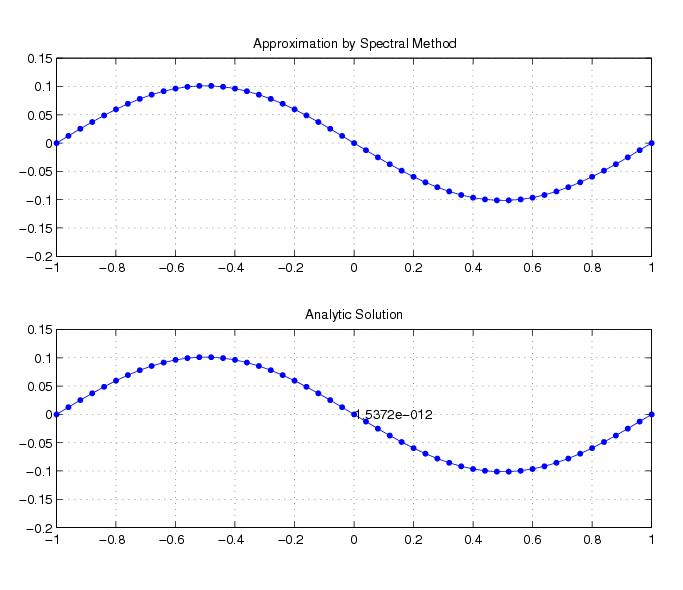
\epsfig{file = Doc-Report_Fwd1D/figs_dn/sinDN_O15.eps, width = 5cm}
    \caption{\label{sinsol1}Numerical and exact solution of equation (\ref{pois_sin1}) with polynomial order $P=15$}
    \end{center}
\end{figure}

\subsubsection {H/P Convergence Test for One-dimensional Solution}

\begin{figure}[h]
\begin{center}
\epsfig{file = Doc-Report_Fwd1D/figs_dn/sinDNhconv.eps, width =8.3cm}
\epsfig{file =Doc-Report_Fwd1D/figs_dn/sinDNpconv.eps,width = 8.3cm}

\caption{\label{sinDNconv1} (Left) Convergence with respect to
discrete $L^{\infty}$ norm as a function of size of elements. This
test is performed using the h-type extension with polynomials of
order 3, 4, and 5 respectively. Error on the Log-Log axis
demonstrates the algebraic convergence of the h-type extension.
(Right) Convergence w.r.t. $L^{\infty}$ norm as a function of size
of polynomial order in semi-Log plot. This shows the exponential
convergence of p-type extension for smooth solution. The tests
were performed for p-type extension with element length $0.2$ and
$0.1$. }
\end{center}
\end{figure}
In this section we present the result of convergence in both $h$
refinement and $p$ refinement with the following steady-state
Poisson differential equation:
\begin{equation}
\label{pois_sin1} \frac{d^2}{dx^2} u(x) = \sin(\pi x),
\end{equation}
for all x in $[-1, 1]$ with zero Dirichlet and Neumann boundary
conditions.


For comparison, the numerical and exact solutions are depicted in
figure (\ref{sinsol1}).

\begin{enumerate}

\item {Convergence of h-type extension for equation (\ref{pois_sin1})}

This test seeks to establish the relation between size of element
and the accuracy of approximation. Utilizing equi-distance
elements, we investigate error. As shown in Figure
(\ref{sinDNconv1}), as elements decrease in size, the accuracy of
the solution improves.

As we see the relationship (\ref{hrelation}) in the theory, the
slope of convergence graph should exhibit slopes of slope 4, 5,
and 6 for the polynomial orders 3, 4, and 5, respectively. The
exact outcome is shown in left table of Table (\ref{hconv2t1}).

\item {Convergence of p-type extension for equation (\ref{pois_sin1})}

Since the exact solution is an infinite sum of polynomial
function, finite order interpolating trial functions cannot reach
ideal convergence. It is also apparant that the convergence will
stagnate before the error reaches machine precision, shown in
right figure of Figure (\ref{sinDNconv1}), the experimented
results support the behavior described in equation
(\ref{hprelation}).

\end{enumerate}

\begin{table}[h]
\centering \caption{\label{hconv2t1} This table shows the
convergence of h-type (left) and p-type (right) resolution control
done above Figure (\ref{sinDNconv1}). Observe that the slopes of
each order $P$ is $P+1$. }
\begin{tabular}{|c|c|c|} \hline
    Polynomial order&Error($L^{\infty}$)&Slope   \\ \hline \hline
    3&$1.1620e-012$ &$4.0024$ \\ \hline
    4&$4.6629e-014$ &$4.9877$ \\ \hline
    5&$9.7367e-014$ &$5.9775$ \\ \hline
\end{tabular}
\hspace{.5in}
\begin{tabular}{|c|c|} \hline
    &\multicolumn{1}{|c|}{Error}\\
    \raisebox{0.5\baselineskip}%
    {Element Size}&($L^{\infty}$) \\ \hline \hline
    0.2&$8.3267e-016$  \\ \hline
    0.1&$6.6613e-016$  \\ \hline
\end{tabular}

\end{table}

\subsection {Approximation of High order Polynomial solving
                                                1-D Poisson Equation}

In this section we construct a polynomial $P_n$ of order $n$
defined on $[0,1]$, which satisfies the following.
\begin{eqnarray*}
 P_n(0) = 0, &P_n(1) = 1 \\
 \frac{d^k}{dx^k}P_n(0) = 0, &\frac{d^k}{dx^k}P_n(1) = 0
\end{eqnarray*}
for all $k = 1, \cdots, n-2$. \\
Then for each $n$, we obtain a polynomial $P_n$ by solving a
system of linear equations having unique solution which determines
the set of coefficients of $P_n$. We will apply the spectral
polynomial solver to approximate the second derivative $Q_{n-2}$
of $P_n$.

Figure \ref{sol1} is showing some samples of solution of
order($n$) $21$.

\begin{problem}
\label{problem2}Consider the following differential equation for
$u(x)$ such that
\begin{equation*}
    \frac{d^2}{dx^2} u(x) = Q_{n-2},
\end{equation*}
for all $x$ in $[0, 1]$. Then the problem is to find approximation
$p(x)$ of $u(x)$ using spectral polynomial method.
\end{problem}

\noindent
%\begin{minipage}[b]{.46\linewidth}
\begin{figure}
  \centering%
  \epsfig{file = figs/0_sol21.eps, %
        height = 6cm}
  \caption{\label{sol1}Solution polynomial of order 21}
%\end{minipage}\hfill
\end{figure}


\subsubsection{Existence of Approximate Solution}

The Figure \ref{crvconvf1} and \ref{crvconvf2} are showing the
result of spectral polynomial method approximating the solution of
Problem \ref{problem2}. The maximum error value in Table
 \ref{crvconv1t} is showing the approximation is within numerically
exact solution tolerance.

\begin{figure}[h]
\begin{center}
\epsfig{file = figs/3_apcrv_app.eps, %
        height = 9cm}
\caption{\label{crvconvf1}Graph showing spectral approximation
satisfying Problem \ref{problem2}}
\end{center}
\end{figure}

\begin{figure}[h]
\begin{center}
\epsfig{file = figs/3_apcrv_err.eps, %
        height = 9cm}
\caption{\label{crvconvf2}Graph showing the error of approximation
in Figure \ref{crvconvf1}}
\end{center}
\end{figure}

\begin{table}[h]
\centering \caption{\label{crvconv1t} Specification of
                              Figure \ref{crvconvf1} and its error}
\begin{tabular}{|c|c|c|c|} \hline
Element Size &Num. of Element &Orders    &Err   \\ \hline \hline
$0.2$        &$5$             &$5, 5, 5, 5, 5$ &$5.7732e-015$ \\
\hline
\end{tabular}
\end{table}


\clearpage
%----------------------------------------------------------------------

\subsubsection{Convergence of Solution in Equidistance and
Uniformly Ordered Elements}

In this section we show the convergence of solutions obtained by
handling orders of basis on each element. We fix the element to be
same size(length) and divide the domain $[0, 1]$ by 5 elements.

Figure \ref{crvconvf3} is the result of convergence to
approximating to a solution of order $5$ in Problem
\ref{problem2}. It shows monotonic decreasing with same similar
slope until the order reaches from $1$ to $4$, and the slope get
stiff between order $4$ and $5$.

Figure \ref{crvconvf4} is that of solution of order $7$. In this
case, the error stops to decrease after the order is larger than
$7$. This part should be considered carefully and need to be made
sure the applicable range of the numerical method.

\begin{figure}[h]
\begin{center}
\epsfig{file = figs/31_equiconv_ord7.eps, %
        height = 9cm}
\caption{\label{crvconvf4}Graph showing convergence of order 7
problem}
\end{center}
\end{figure}

\begin{figure}[h]
\begin{center}
\epsfig{file = figs/explicitdd_od10_int5_10.eps, %
        height = 9cm}
\caption{\label{crvconvf4}Graph showing convergence of order
10(explicit) problem with 5/10 elements}
\end{center}
\end{figure}

%\clearpage
%----------------------------------------------------------------------

\subsubsection{Test of Convergence of Solution in Variable Ordered
Elements}

According to the idea that the solution need to be carefully
approximated specially in the center of the curve, we assign
different orders by the position of elements. I tested 2 cases.
The one is to variate 3 elements in center among 5 elements. The
other is to variate 1 element in the exact center of all elements.

Figure \ref{crvconvf5} is the first case with 3 different orders
at the $2$ ends of elements. Since it is based on the solution of
order $5$, the orders in 3 center elements moves from $1$ to $5$.

Figure \ref{crvconvf6} is the same as Figure \ref{crvconvf5}
except that it is based on solution of order 7 problem and the
orders at the center elements varies from 1 to 7.


\begin{figure}[h]
\begin{center}
\epsfig{file = figs/32_variconv_ordppp5.eps, %
        height = 9cm}
\caption{\label{crvconvf5}Graph showing convergence of order 5
problem}
\end{center}
\end{figure}

\begin{figure}[h]
\begin{center}
\epsfig{file = figs/32_variconv_ordppp7.eps, %
        height = 9cm}
\caption{\label{crvconvf6}Graph showing convergence of order 7
problem}
\end{center}
\end{figure}

Figure \ref{crvconvf7} and Figure \ref{crvconvf8} are the same as
\ref{crvconvf5} and \ref{crvconvf6} except that these have the
element that varies only a center element. The 2 different control
of orders on each element doesn't give out much different error
movement. This means choosing wise orders in each element can save
time of computing since the lower is the order, the faster does
the system solve.

\begin{figure}[h]
\begin{center}
\epsfig{file = figs/32_variconv_ordp5.eps, %
        height = 9cm}
\caption{\label{crvconvf7}Graph showing convergence of order 5
problem}
\end{center}
\end{figure}

\begin{figure}[h]
\begin{center}
\epsfig{file = figs/32_variconv_ordp7.eps, %
        height = 9cm}
\caption{\label{crvconvf8}Graph showing convergence of order 7
problem}
\end{center}
\end{figure}


%\clearpage
%\vspace*{3cm}
\clearpage
\section{Spectral Fourier Method on 2-dimensional Annulus}

\subsection{Mathematical Formulations}
%\{ {\it  sp1d\_ch2.tex} \}

\subsection{Poisson Equation in Polar Coordinates and Basis Functions}

We formulate the Generalized Poisson problem on an annulus $[a, b]\times[0, 2\pi]$, $a > 0$ under the periodic solution $u$ as follows:
\begin{eqnarray}\label{genpois}
-\left[\frac{\partial}{\partial r} (\sigma(r,\theta) \frac{\partial}{\partial r}) + \frac{1}{r} (\sigma(r,\theta) \frac{\partial}{\partial r}) + \frac{1}{r^2}\frac{\partial}{\partial \theta} (\sigma(r,\theta)  \frac{\partial}{\partial \theta})\right] u(r, \theta) = f(r, \theta),\\
\mbox{with periodicity of }u, \;\;\; u(r,0) = u(r,2\pi),
\end{eqnarray}
where $r \in [a, b]$ and $\theta \in [0, 2 \pi]$. The boundary conditions for this domain is given by
\begin{equation}
u(a,\theta) = {\mathcal G}_D(\theta), \hspace{1in} \frac{\partial}{\partial r} u(b,\theta) = {\mathcal G}_N(\theta),
\end{equation}
where $\theta \in [0,2\pi]$.

\vspace{0.1in}
The representation of approximation of $u$ is guaranteed by Weierstrass theorem:
\begin{equation}\label{truncapp}
u(r,\theta) = \sum_{j=0}^{N_r} \sum_{k=-N_\theta/2+1}^{N_\theta/2} \hat{u}_{jk} \phi_j(r) e^{ik\theta},
\end{equation}
where $r \in [a, b]$ and $\theta \in [0, 2 \pi]$ for the global degree of freedom $N_r$ and $N_{\theta}$ on $\hat{u}_{jk}$'s.

\vspace{0.1in}
The basis function $\{\phi_j\}_{j=0}^{N_r}$ at (\ref{truncapp}) are defined as modified Jacobi polynomials defined in \cite{Karniadarkis}, \cite{Choe}.

\vspace{0.1in}
As a review of discrete Fourier transform in $N$-point grid described in \cite{Trefethen}, the formula for the discrete Fourier transform for $\{v_j\}$ is
\begin{equation}
\hat{v}_k = h \sum_{j=1}^{N} e^{-ikx_j}v_j, \;\; k = -\frac{N}{2}+1, \ldots , \frac{N}{2},
\end{equation}
where $x_j = j\frac{2\pi}{N}$ and the inverse discrete Fourier transform for $\{\hat{v}_k\}$ is given by
\begin{equation}
v_j = \frac{1}{2\pi}\sum_{k = -N/2+1}^{Nr/2}e^{ikx_j}\hat{v}_k,\;\; j = 1, \ldots, N.
\end{equation}


\subsection{Formulation of Spectral Polynomial and Fourier Methods}

In this project, we assume the conductivity term $\sigma$ in (\ref{genpois}) to be only dependent of variables showing the radius domain as we multiply $r^2$ in each side of (\ref{genpois}). Then the Poisson equation and its modified form of polar coordinate was obtained as follows:
\begin{eqnarray}
-\left[r^2 \frac{\partial}{\partial r} (\sigma(r) \frac{\partial}{\partial r}) + r \sigma(r) \frac{\partial}{\partial r} + \sigma(r) \frac{\partial^2}{\partial \theta^2}\right] u(r, \theta) = r^2 f(r, \theta).
\end{eqnarray}

\vspace{0.1in}
To apply Galerkin method, test functions are of the form:
\begin{equation}
\phi_p(r) e^{iq\theta}, \hspace{.5in} p=0,\ldots,N_r, \;\; q = -\frac{N_\theta}{2}+1,\ldots,\frac{N_\theta}{2}.
\end{equation}

\vspace{0.1in}
We have the weak form of the equation:
\begin{equation}\label{galeqn}
-\langle  r^2 \frac{\partial}{\partial r} (\sigma \frac{\partial}{\partial r}u) + r \sigma \frac{\partial}{\partial r}u + \sigma \frac{\partial^2}{\partial \theta^2}u, \phi_p e^{iq\theta} \rangle = \langle r^2 f, \phi_p e^{iq\theta} \rangle.
\end{equation}

\vspace{0.1in} Define $T_i, i = 1,\ldots,4$ as follows
\begin{eqnarray}
T_1 &=& \int_{0}^{2\pi} \int_{a}^{b} \phi_p e^{iq\theta} r^2 \frac{\partial}{\partial r}\left[\sigma(r) \frac{\partial}{\partial r}u(r, \theta)\right] dr d\theta,\\
T_2 &=& \int_{0}^{2\pi} \int_{a}^{b} \phi_p e^{iq\theta} r \sigma(r) \frac{\partial}{\partial r}u(r, \theta) dr d\theta,\\
T_3 &=& \int_{0}^{2\pi} \int_{a}^{b} \phi_p e^{iq\theta} \sigma(r) \frac{\partial^2}{\partial \theta^2}u(r, \theta) dr d\theta,\\
\mbox{and} \hspace{.5in}T_4 &=& \int_{0}^{2\pi} \int_{a}^{b} \phi_p e^{iq\theta} r^2 f(r, \theta) dr d\theta
\end{eqnarray}

Then we can represent (\ref{galeqn}) to be:
\begin{equation}\label{smpeqn}
- T_1 - T_2 - T_3 = T_4.
\end{equation}

We can obtain boundary term by integration by part on $T_1$
\begin{eqnarray}
T_1 &=& \int_0^{2\pi}e^{iq\theta} \left[ r^2\sigma(r)\frac{\partial}{\partial r}u(r,\theta)\phi_p(r)\right]_a^b d\theta \\
&-&2 \int_0^{2\pi}\int_a^b e^{iq\theta} r \sigma(r)\frac{\partial}{\partial r}u(r,\theta)\phi_p(r)drd\theta \\
&-& \int_0^{2\pi}\int_a^b e^{iq\theta} r^2\sigma(r)\frac{\partial}{\partial r}u(r,\theta) \frac{d}{dr}\phi_p(r)drd\theta.
\end{eqnarray}

Then the right hand side of (\ref{smpeqn}) becomes
\begin{eqnarray}\label{rhseqn1}
- T_1 - T_2 - T_3 &=& - \int_0^{2\pi}e^{iq\theta} \left[ r^2\sigma(r)\frac{\partial}{\partial r}u(r,\theta)\phi_p(r)\right]_a^b d\theta \\
&+& \int_0^{2\pi}\int_a^b e^{iq\theta} r \sigma(r) \frac{\partial}{\partial r}u(r,\theta)\phi_p(r)drd\theta \\
&+& \int_0^{2\pi}\int_a^b e^{iq\theta} r^2 \sigma(r) \frac{\partial}{\partial r}u(r,\theta) \frac{d}{dr}\phi_p(r)drd\theta \\
&-& \int_0^{2\pi}\int_a^b e^{iq\theta} \sigma(r) \frac{\partial^2}{\partial \theta^2}u(r, \theta) \phi_p(r) dr d\theta
\end{eqnarray}

By using (\ref{truncapp}) and the orthogonal property in
$\{e^{ik\theta}\}k = -\frac{N_\theta}{2}+1,\ldots,\frac{N_\theta}{2}$,
we can simplify (\ref{rhseqn1}) as follows:

\begin{eqnarray}\label{rhseqn2}
- T_1 - T_2 - T_3 &=& - \int_0^{2\pi}e^{iq\theta} \left[ r^2\sigma(r)\frac{\partial}{\partial r}u(r,\theta)\phi_p(r)\right]_a^b d\theta \\
&+& 2\pi \sum_{j=0}^{N_\theta} \hat{u}_{jq} \int_a^b r \sigma(r) \frac{d}{dr} \phi_j(r) \phi_p(r) dr \\
&+& 2\pi \sum_{j=0}^{N_\theta} \hat{u}_{jq} \int_a^b r^2 \sigma(r) \frac{d}{dr} \phi_j(r) \frac{d}{dr}\phi_p(r) dr \\
&+& 2\pi \sum_{j=0}^{N_\theta} \hat{u}_{jq} q^2 \int_a^b \sigma(r) \phi_j(r) \phi_p(r) dr.
\end{eqnarray}


Let us define the following matrices:
\begin{eqnarray}
({\bf M}_1)_{jp} & = & \int_a^b r \sigma(r) \frac{d}{dr} \phi_j(r) \phi_p(r) \;dr  \\
({\bf M}_2)_{jp} & = & \int_a^b r^2 \sigma(r) \frac{d}{dr} \phi_j(r) \frac{d}{dr} \phi_p(r) \;dr  \\
({\bf M}_3)_{jp} & = & \int_a^b \sigma(r) \phi_j(r) \phi_p(r) \; dr,
\end{eqnarray}
where $j, p = 0, \ldots, N_\theta$.

Now the form $T_4$ is as follows.

\begin{eqnarray}
T_4 &=& \int_a^b \int_0^{2\pi} \phi_p(r) e^{iq\theta} r^2 f(r,\theta) d\theta dr \\
    &=& \int_a^b r^2\phi_p(r) \int_0^{2\pi} f(r,\theta) e^{iq\theta} d\theta dr \\
\end{eqnarray}

For given $r$, the Discrete Fourier Transform for $f(r, \theta)$ is defined by
\begin{equation}
f(r, \theta_\tau) = \frac{1}{2\pi} \sum_{k=-N_\theta/2+1}^{N_\theta/2} e^{ik\theta_\tau} \widehat{f(r)}_k
\end{equation}

where
\begin{equation}
\widehat{f(r)}_k = \frac{2\pi}{N_\theta} \sum_{j=1}^{N_\theta} e^{-ik\theta_j} f(r, \theta_j)
\end{equation}
with $ k \in \{-\frac{N_\theta}{2}+1, \cdots, \frac{N_\theta}{2}\}$ and $\theta_j \in \{ \frac{2\pi}{N_\theta}, \cdots, 2\pi  \}$.  

Then
\begin{center}
\begin{eqnarray}
T_4&=& \int_a^b r^2\phi_p(r) \int_0^{2\pi} \frac{1}{2\pi} \sum_{k=-N_\theta/2+1}^{N_\theta/2} e^{ik\theta} \widehat{f(r)}_k e^{iq\theta} d\theta dr \\
%&=& \int_a^b r^2\phi_p(r) \sum_{k=-N_\theta/2+1}^{N_\theta/2} \widehat{f(r)}_k \frac{1}{2\pi} \int_0^{2\pi}  e^{ik\theta} e^{iq\theta} d\theta dr \\
%&=& \int_a^b r^2\phi_p(r) \sum_{k=-N_\theta/2+1}^{N_\theta/2} \widehat{f(r)}_k \delta_{k,q} dr\\
&=& \int_a^b r^2\phi_p(r) \widehat{f(r)}_q dr.
%&=& \sum_\sigma w_\sigma r_\sigma^2\phi_p(r_\sigma) \widehat{f(r_\sigma)}_q.
\end{eqnarray}
\end{center}


Since we have this relation $- T_1 - T_2 - T_3 = T_4$,

\begin{eqnarray}
 2\pi \sum_{j=0}^{N_\theta} \hat{u}_{jq} {M_1}_{jp}
+ 2\pi \sum_{j=0}^{N_\theta} \hat{u}_{jq} {M_2}_{jp} 
+ 2\pi \sum_{j=0}^{N_\theta} \hat{u}_{jq} q^2 {M_3}_{jp} 
= \int_a^b r^2\phi_p(r) \widehat{f(r)}_q dr \\
+ b^2\sigma(b) \phi_p(b) \int_0^{2\pi}e^{iq\theta} {\mathcal G}_N(\theta) d\theta 
- a^2\sigma(a) \phi_p(a) \int_0^{2\pi}e^{iq\theta} \frac{\partial}{\partial r}u(a,\theta) d\theta
\end{eqnarray}
where $j, p = 0, \ldots, N_r$.

 At this stage, we can apply Fourier transform to the integral term having ${\mathcal G}_N$ and the same idea as 
one-dimensional case to each term about boundary conditions.


\subsection{Experiment Results}
%\{ {\it  sp1d\_ch3\_1.tex} \}

\subsection {H/P Convergence Test for Two-dimensional Solution}

In this section we present the result of convergence in both $h$ refinement and $p$ refinement with the following steady-state Poisson differential equation:
\begin{equation}
\label{pois_sin}
-r^2 \frac{\partial}{\partial r} (\sigma \frac{\partial}{\partial r}u) - r \sigma \frac{\partial}{\partial r}u - \sigma \frac{\partial^2}{\partial \theta^2}u = r \cos \theta \left[ -4 r \pi \cos S_r + \{4\pi^2 + 1\} \sin S_r \right],
\end{equation}
for all $r \in [1, 2], \theta \in [0, 2\pi]$ with $\sigma(r) = r$. The analytic solution is known as 
\begin{equation}
u(r, \theta) = \sin S_r \cos \theta,
\end{equation}
where $S_r = 2\pi (r-1) - \pi$.

The numerical and exact solutions by the solver we developed is shown in figure (\ref{sinsol}).

\begin{figure}[h]
    \begin{center}
    \epsfig{file = figs_dn/sinDN_e10_t8.eps, width = 5cm} %Error: 4.7740e-15
    \epsfig{file = figs_dn/sinDN_e10_t8_1.eps, width = 5cm}
    \caption{\label{sinsol}Numerical and exact solution of equation (\ref{pois_sin}) with polynomial order $P=10$, $10$ equidistance elements. This gives the error 4.7740e-15 to the exact solution}
    \end{center}
\end{figure}

\begin{figure}[h]
    \begin{center}
    \epsfig{file = figs_dn/sinDNhconv.eps, width = 8.3cm}
    \epsfig{file = figs_dn/sinDNpconv.eps, width = 8.3cm}
    \caption{\label{sinDNconv}
(Left)Convergence with respect to discrete $L^{\infty}$ norm as a function of size of elements. This test is performed using the h-type extension with fixed polynomial order 5 and 6 respectively. Error on the Log-Log axis is demonstrating the algebraic convergence of the h-type extension.
(Right)Convergence w.r.t. $L^{\infty}$ norm as a function of size of polynomial order in semi-Log plot. It shows the exponential convergence of p-type extension for smooth solution. Two tests are performed for p-type extension with element length $0.2$ and $0.1$.
}
\end{center}
\end{figure}


\begin{table}[h]
\centering \caption{\label{hconv2t} This table shows the convergence of h-type (left) and p-type (right) resolution control done above Figure (\ref{sinDNconv}). We can see the slopes of each order $P$ is $P+1$ }
\begin{tabular}{|c|c|c|} \hline
    Polynomial order&Error($L^{\infty}$)&Slope   \\ \hline \hline
    5&$9.3603e-013$ &$5.9406$ \\ \hline
    6&$8.6542e-014$ &$6.9402$ \\ \hline
\end{tabular}
\hspace{.5in}
\begin{tabular}{|c|c|} \hline
    Element Size&Error($L^{\infty}$)\\ \hline
    0.2&$1.9385e-012$  \\ \hline
    0.1&$3.4611e-013$  \\ \hline
\end{tabular}

\end{table}

%\{ {\it  sp1d\_ch3\_2.tex} \}

\subsection {High order Polynomial Solution and Its Convergence}

In this section we construct a polynomial $P_n$ of order $n$ defined on $[0,1]$, which satisfies the following.
\begin{eqnarray}
\label{pois_scrv}
    P_n(0) = 0, &P_n(1) = 1 \\
    \frac{d^k}{dx^k}P_n(0) = 0, &\frac{d^k}{dx^k}P_n(1) = 0
\end{eqnarray}
for all $k = 1, \cdots, n-2$. \\
Then for each $n$, we obtain a polynomial $P_n$ by solving a system of linear equations having unique solution which determines the set of coefficients of $P_n$. We will apply the spectral polynomial solver to approximate the second derivative $Q_{n-2}$ of $P_n$.

\begin{figure}[h]
    \begin{center}
    \epsfig{file = figs_dn/ScrvH5_A.eps, width = 5cm}
    \epsfig{file = figs_dn/ScrvH5_N.eps, width = 5cm}
    \caption{\label{scrvsol}Example of curve that satisfies conditions (\ref{pois_scrv}) with polynomial order $n=7, 9, 12, 14, 15$. The error is $2.9239e-8$}
    \end{center}
\end{figure}

We will investigate the convergences by the h-type, p-type extension of trial functions below.

\begin{problem}
Consider the following differential equation for $u(x)$ such that
\begin{equation}
\label{poi_poly}
-r^2 \frac{\partial}{\partial r} (\sigma \frac{\partial}{\partial r}u) - r \sigma \frac{\partial}{\partial r}u - \sigma \frac{\partial^2}{\partial \theta^2}u = e^{-(r-1)^2}\{P_n(r) + (2r^2(r-1)-r)P_n'(r) - r^2 P_n''(r)\} \cos \theta,
\end{equation}
for all $r$ in $[0.1, 1.1]$ with $\sigma(r) = e^{-(r-1)^2}$. Then we have the exact solution as follows.
\begin{equation}
u(r, \theta) = P_n(r) \cos \theta
\end{equation}
where $r$ in $[0.1, 1.1]$ and $\theta$ in $[0, 2\pi]$.
\end{problem}

Note that the accuracy of this interpolation satisfying equations (\ref{pois_scrv}) is dependent on the stability of matrix that defines the coefficients of interpolants. We used the Legendre basis function which is known to be more stable than monomials. In spite of this, there exists interpolation error close to $e^{-13}$. This cause the same amount of convergence error in p-type extension mode shown in right of Figure (\ref{ScrvconvDN}) and Table (\ref{hconv2t}).

\begin{figure}[h]
\begin{center}
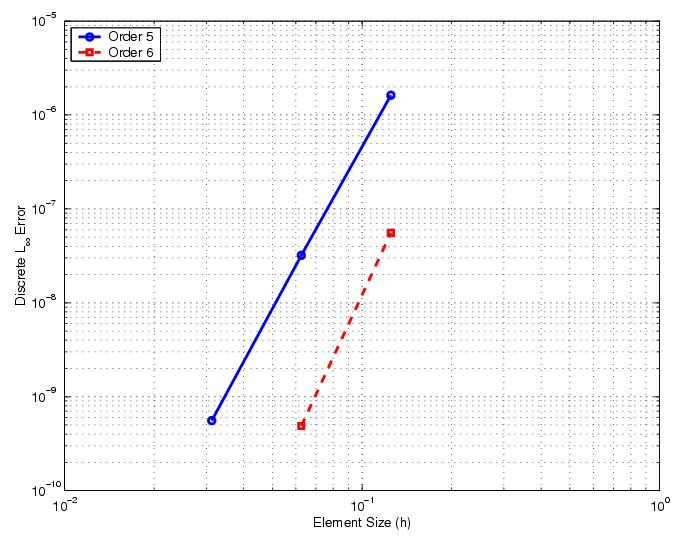
\epsfig{file = figs_dn/ScrvHconv.eps, width = 8.3cm}
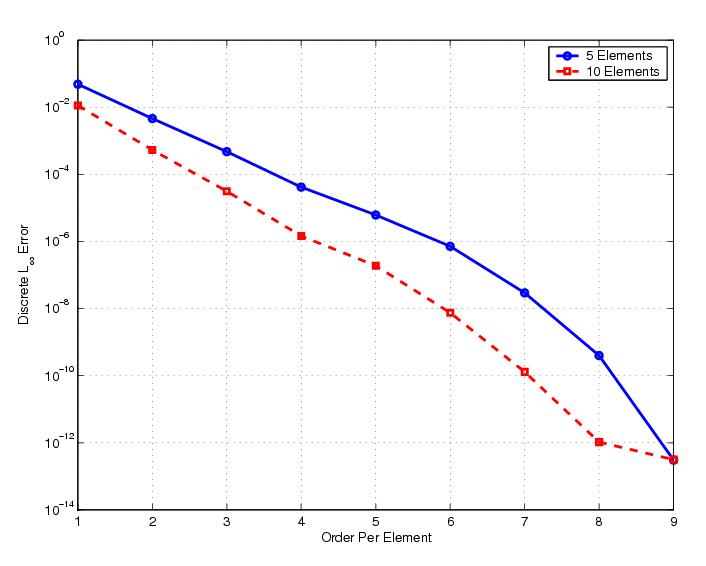
\epsfig{file = figs_dn/ScrvPconv.eps, width = 8.3cm}
\caption{\label{ScrvconvDN}
(Left)Convergence with respect to discrete $L^{\infty}$ norm as a function of size of elements. This test is performed using the h-type extension with fixed polynomial order 3, 4, and 5 respectively. Error on the Log-Log axis is demonstrating the algebraic convergence of the h-type extension.
(Right)Convergence w.r.t. $L^{\infty}$ norm as a function of size of polynomial order in semi-Log plot. It shows the exponential convergence of p-type extension for smooth solution. Two tests are performed for p-type extension with element length $0.2$ and $0.1$.
}
\end{center}
\end{figure}

\begin{table}[h]
\centering \caption{\label{hconv2t} This table shows the convergence of h-type resolution control done above Figure (\ref{ScrvconvDN}). We can see the slopes of each order $P$ is $P+1$ }
\begin{tabular}{|c|c|c|} \hline
    Polynomial order&Error($L^{\infty}$)&Slope   \\ \hline \hline
    5&$8.5305e-012$ &$5.7556$ \\ \hline
    6&$4.7180e-012$ &$6.8332$ \\ \hline
\end{tabular}
\hspace{.5in}
\begin{tabular}{|c|c|} \hline
    {Element Size}&Error($L^{\infty}$) \\ \hline \hline
    0.2&$9.0616e-13$  \\ \hline
    0.1&$9.4747e-13$ \\ \hline
\end{tabular}
\end{table}


\clearpage
\section{Conclusion}
%\clearpage
%\{ {\it  sp1d\_ch4\_1.tex} \}

Throughout this project, we investigate the application of
Spectral Polynomial Element Method to Poisson equations. We also
compared the  of h/p convergence properties of the method to the
classical finite element method. The Galerkin method allows
incorporation of the weak solution into the formulation for the
problem as system of linear equations which can be solved
numerically.

The Spectral element solver for one dimensional Poisson equation
with Dirichlet and Neumann boundary conditions, with high-order
solutions exhibited much accurate solutions which were hard to get
acceptable convergence in a given time and resolution of domain in
past.

For the future study, we would like deal with problems regarding:

\begin{itemize}
\item
development multi-dimensional solver.
\item
obtaining solutions to various natural phenomena that obey
governing equations.
\item
utilizing the method in the ill-posed problem. By using certain
technique that we can approximate the solution, we can also apply
this method to the problem and compare with other method in that
situation.
\end{itemize}


%\end{spacing}
%------------------------------------------------------------------------------
%   BIBLIOGRAPHY
%\clearpage

%\{ {\it  sp1d\_chbib.tex} \}

\begin{thebibliography}{9}

\bibitem{Karniadarkis}{\bf Spectral/Hp Element Methods for Cfd}
        George Em Karniadakis, Spencer J. Sherwin, \/
        Oxford Univ Press, 1999.

\bibitem{Trefethen}{\bf Spectral Methods in MATLAB}
        Lloyd N. Trefethen, \/
        Society for Industrial and Applied Mathematics, 2001.

\bibitem{Johnson}{\bf Lecture note of Advanced Methods in Scientific Computing}
        Christopher R. Johnson, \/
        School of Computing, University of Utah, 2002.


\bibitem{Chen}{\bf A direct spectral collocation Poisson solver in polar and cylindrical
coordinates},
        Chen HL. Su YH. and Shizgal BD., \/
        Journal of Computational Physics. 160(2), 453-469 (2000).


\end{thebibliography}



%-------------------------------------------------------------------------------
%   APPENDIX


\end{document}
